\documentclass[11pt,a4paper]{article}
\usepackage[margin=21mm,headheight=16pt]{geometry}
\usepackage{fontspec}\setmainfont{Noto Serif}\setsansfont{Noto Sans}\setmonofont{Noto Sans Mono}
\usepackage{polyglossia}\setdefaultlanguage{turkish}
\usepackage{amsmath,amssymb,mathtools,graphicx,xcolor,booktabs,tabularx,array,enumitem}
\usepackage[most]{tcolorbox}\usepackage{fancyhdr,titlesec,needspace}
\usepackage[unicode,hidelinks,breaklinks]{hyperref}\usepackage{bookmark}
\definecolor{ink}{HTML}{18233A}\definecolor{accent}{HTML}{545AC4}\definecolor{green}{HTML}{087E66}\definecolor{paper}{HTML}{F3F5FA}
\color{ink}\setlength{\parindent}{0pt}\setlength{\parskip}{7pt}\linespread{1.10}
\setlength{\emergencystretch}{3em}\allowdisplaybreaks
\setlist{topsep=4pt,itemsep=4pt,leftmargin=*}
\pagestyle{fancy}\fancyhf{}\fancyhead[L]{\sffamily\small MÜHENDİSLİK MATEMATİĞİ}\fancyhead[R]{\sffamily\small Ders çalışma notları}\fancyfoot[L]{\sffamily\scriptsize Fotoğraflar + müfredat | 8 Kasım 2026}\fancyfoot[R]{\sffamily\thepage}
\titleformat{\section}{\Large\sffamily\bfseries\color{accent}}{\thesection}{.6em}{}
\titleformat{\subsection}{\large\sffamily\bfseries}{\thesubsection}{.6em}{}
\tcbset{enhanced,breakable,boxrule=.4pt,arc=2mm,left=3mm,right=3mm,top=2mm,bottom=2mm,before skip=8pt,after skip=8pt,fonttitle=\sffamily\bfseries,colback=paper,colframe=accent,coltitle=white}
\newcommand{\notebox}[2]{\begin{tcolorbox}[title={#1},colframe=accent!70!black]#2\end{tcolorbox}}
\hypersetup{pdfauthor={Mühendislik Matematiği Çalışma Atölyesi},pdfsubject={Ders fotoğrafları ve altı başlıklı müfredata göre özgün Türkçe çalışma notları}}
\begin{document}

\hypersetup{pdftitle={Üç boyutlu uzay ve vektörler}}
{\sffamily\small\color{accent} ÇALIŞMA ATÖLYESİ / KONU 01\par}
\vspace{8mm}
{\Huge\sffamily\bfseries\raggedright\hyphenpenalty=10000 Üç boyutlu uzay ve vektörler\par}
\vspace{3mm}
{\large Koordinatlar, norm, birim vektör, skaler ve vektörel çarpım, izdüşüm ve lineer bağımsızlık.\par}
\vspace{4mm}\hrule\vspace{4mm}\subsection*{Bu bölümün hedefleri}\begin{itemize}
\item Nokta ile vektör arasındaki farkı açıklamak; uzunluk ve yön bulmak.
\item Bir soruda skaler çarpım mı vektörel çarpım mı gerektiğini seçmek.
\item Alan, hacim, izdüşüm ve bağımsızlık problemlerini çözmek.\end{itemize}
{\small\tableofcontents}\clearpage
\section{Uzayı koordinatlarla okumak}
Bir noktayı belirtmek için konum, bir vektörü belirtmek için büyüklük ve yön gerekir. Sağ elli Kartezyen sistemde \(P=(x,y,z)\) noktasının koordinatları sırasıyla \(yz\), \(xz\), \(xy\) düzlemlerine göre işaretli konumunu anlatır. \(xy\) düzlemi \(z=0\), \(xz\) düzlemi \(y=0\), \(yz\) düzlemi \(x=0\) ile tanımlanır. Üç koordinatın işaretleri uzayı sekiz bölgeye ayırır.

\(A\) noktasından \(B\) noktasına giden vektör her koordinatta son eksi ilk alınarak bulunur. Başlangıç noktası değişse bile aynı büyüklük ve yönü koruyan oklar aynı serbest vektörü temsil eder. Buna karşılık \(\overrightarrow{OA}\), başlangıcı orijin olduğu için konum vektörüdür.


{\small\[
\overrightarrow{AB}=(x_B-x_A,y_B-y_A,z_B-z_A),\qquad d(A,B)=\sqrt{(x_B-x_A)^2+(y_B-y_A)^2+(z_B-z_A)^2}.
\]}
\notebox{Ön bilgi}{Tek değişkenli türev ve integral kuralları sonraki bölümlerde kullanılacak. Bu ilk bölüm için Pisagor bağıntısı, determinant ve temel trigonometri yeterlidir.}
\section{Vektör işlemleri, norm ve birim vektör}
\(\mathbf u=(u_1,u_2,u_3)\) ve \(\mathbf v=(v_1,v_2,v_3)\) için toplama bileşen bileşen yapılır. \(\lambda\mathbf u\) uzunluğu \(|\lambda|\) katına çıkarır; \(\lambda<0\) ise yönü ters çevirir. Standart baz \(\mathbf i=(1,0,0),\mathbf j=(0,1,0),\mathbf k=(0,0,1)\) olduğundan \(\mathbf u=u_1\mathbf i+u_2\mathbf j+u_3\mathbf k\) yazılır.


{\small\[
\mathbf u+\mathbf v=(u_1+v_1,u_2+v_2,u_3+v_3),\quad \|\mathbf u\|=\sqrt{u_1^2+u_2^2+u_3^2},\quad \widehat{\mathbf u}=\frac{\mathbf u}{\|\mathbf u\|}\quad(\mathbf u\ne\mathbf0).
\]}
\Needspace{10\baselineskip}\begin{tcolorbox}[title={Örnek 1.1 | Birim vektör},colframe=accent]\(\mathbf u=(3,4)\) yönündeki birim vektörü bulunuz.
\par\vspace{1mm}{\scriptsize\sffamily Ders fotoğrafından | \nolinkurl{IMG-20261009-WA0026.jpg}}\end{tcolorbox}
\begin{tcolorbox}[title={Adım adım çözüm},colback=green!3!white,colframe=green]\begin{enumerate}
\item Önce norm alınır: \(\|\mathbf u\|=\sqrt{9+16}=5\).
\item Her bileşeni 5 ile bölünce \(\widehat{\mathbf u}=(3/5,4/5)\) elde edilir. Norm kontrolü \(9/25+16/25=1\) verir. Ters yöndeki birim vektör bunun negatifidir.
\end{enumerate}\end{tcolorbox}
\notebox{Sıfır vektörü}{\(\mathbf0\) için yön ve birim vektör tanımlanmaz. Birimleştirme yapmadan önce paydanın sıfır olmadığını kontrol et.}
\section{Skaler çarpım, açı ve diklik}
Skaler çarpım iki vektörün aynı doğrultuda ne kadar bileşeni bulunduğunu ölçer; sonucu sayıdır. Bileşen formülü hesaplamada, geometrik formül açı yorumunda kullanılır. Sıfır olmayan vektörler için çarpım pozitifse dar, negatifse geniş, sıfırsa dik açı vardır.


{\small\[
\mathbf u\cdot\mathbf v=u_1v_1+u_2v_2+u_3v_3=\|\mathbf u\|\|\mathbf v\|\cos\theta,\qquad \cos\theta=\frac{\mathbf u\cdot\mathbf v}{\|\mathbf u\|\|\mathbf v\|}.
\]}
\Needspace{10\baselineskip}\begin{tcolorbox}[title={Örnek 1.2 | Dersteki açı sorusu},colframe=accent]\(\mathbf u=(2,-1,3)\) ve \(\mathbf v=(1,4,2)\) dik midir? \(\cos\theta\) nedir?
\par\vspace{1mm}{\scriptsize\sffamily Ders fotoğrafından | \nolinkurl{IMG-20261009-WA0032.jpg}}\end{tcolorbox}
\begin{tcolorbox}[title={Adım adım çözüm},colback=green!3!white,colframe=green]\begin{enumerate}
\item \(\mathbf u\cdot\mathbf v=2-4+6=4\). Çarpım sıfır olmadığından dik değildirler.
\item \(\|\mathbf u\|=\sqrt{14}\), \(\|\mathbf v\|=\sqrt{21}\). Dolayısıyla \(\cos\theta=4/\sqrt{294}\). Pozitif sonuç açının dar olduğunu doğrular.
\end{enumerate}\end{tcolorbox}
Yön kosinüsleri, vektörün pozitif koordinat eksenleriyle yaptığı açıların kosinüsleridir. \(\cos\alpha=u_1/\|\mathbf u\|\), \(\cos\beta=u_2/\|\mathbf u\|\), \(\cos\gamma=u_3/\|\mathbf u\|\) ve \(\cos^2\alpha+\cos^2\beta+\cos^2\gamma=1\). Bu bağıntı birim vektör kontrolünün başka bir biçimidir.

\notebox{Vektör açısı ve doğru açısı}{İki vektörün açısı \([0,\pi]\) aralığındadır. İki yönsüz doğru arasındaki küçük açı için paydaki skaler çarpımın mutlak değeri kullanılır.}
\section{İzdüşüm: bir vektörü iki parçaya ayırmak}
Bir kuvveti eğim boyunca ve eğime dik bileşenlerine ayırırken izdüşüm kullanılır. \(\mathbf u\) vektörünün \(\mathbf v\) doğrultusundaki işaretli skaler bileşeni bir sayıdır; vektörel izdüşümü ise bu sayı ile \(\widehat{\mathbf v}\) çarpılarak elde edilir.


{\small\[
\operatorname{comp}_{\mathbf v}\mathbf u=\frac{\mathbf u\cdot\mathbf v}{\|\mathbf v\|},\qquad \operatorname{proj}_{\mathbf v}\mathbf u=\frac{\mathbf u\cdot\mathbf v}{\|\mathbf v\|^2}\mathbf v.
\]}
\(\mathbf u_{\perp}=\mathbf u-\operatorname{proj}_{\mathbf v}\mathbf u\) kalanı \(\mathbf v\) ile diktir. Kontrol için kalanla \(\mathbf v\) skaler çarpılır. İşaretli bileşen negatif olabilir; izdüşümün uzunluğu istendiğinde mutlak değer alınır.

\Needspace{10\baselineskip}\begin{tcolorbox}[title={Örnek 1.3 | İzdüşüm hesabı},colframe=accent]\(\mathbf u=(2,1,2)\) vektörünü \(\mathbf v=(1,0,1)\) doğrultusuna izdüşürünüz.
\par\vspace{1mm}{\scriptsize\sffamily Pekiştirme}\end{tcolorbox}
\begin{tcolorbox}[title={Adım adım çözüm},colback=green!3!white,colframe=green]\begin{enumerate}
\item \(\mathbf u\cdot\mathbf v=4\), \(\|\mathbf v\|^2=2\). Bu yüzden izdüşüm \(2(1,0,1)=(2,0,2)\).
\item Dik kalan \((0,1,0)\) olur ve \((0,1,0)\cdot(1,0,1)=0\). Skaler bileşen \(4/\sqrt2=2\sqrt2\).
\end{enumerate}\end{tcolorbox}
\begin{center}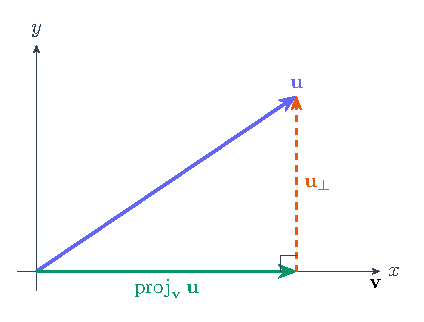
\includegraphics[width=.94\linewidth,height=65mm,keepaspectratio]{../assets/figures/projection.pdf}\par{\small\sffamily İzdüşüm, vektörü bir doğrultuya paralel ve o doğrultuya dik iki bileşene ayırır.}\end{center}
\section{Vektörel çarpım ve alan}
Vektörel çarpım \(\mathbb R^3\) içinde her iki girdiye de dik bir vektör üretir. Yönü sağ el kuralıyla belirlenir. Sıra değişirse işaret değişir; bu yüzden determinant açılımındaki orta bileşenin eksi işaretine dikkat edilir.


{\small\[
\mathbf u\times\mathbf v=\begin{vmatrix}\mathbf i&\mathbf j&\mathbf k\\u_1&u_2&u_3\\v_1&v_2&v_3\end{vmatrix}=(u_2v_3-u_3v_2,\ u_3v_1-u_1v_3,\ u_1v_2-u_2v_1).
\]}

{\small\[
\|\mathbf u\times\mathbf v\|=\|\mathbf u\|\|\mathbf v\|\sin\theta,\qquad A_{\rm paralelkenar}=\|\mathbf u\times\mathbf v\|,\quad A_{\text{üçgen}}=\frac12\|\mathbf u\times\mathbf v\|.
\]}
\Needspace{10\baselineskip}\begin{tcolorbox}[title={Örnek 1.4 | Tahtadaki vektörel çarpım},colframe=accent]\(\mathbf u=(1,2,3)\), \(\mathbf v=(2,0,1)\) için \(\mathbf u\times\mathbf v\) bulunuz.
\par\vspace{1mm}{\scriptsize\sffamily Ders fotoğrafından | \nolinkurl{IMG-20261023-WA0029.jpg}}\end{tcolorbox}
\begin{tcolorbox}[title={Adım adım çözüm},colback=green!3!white,colframe=green]\begin{enumerate}
\item Bileşenler \((2\cdot1-3\cdot0,\,3\cdot2-1\cdot1,\,1\cdot0-2\cdot2)\) şeklindedir. Sonuç \((2,5,-4)\).
\item Diklik kontrolleri: \((2,5,-4)\cdot(1,2,3)=2+10-12=0\) ve \((2,5,-4)\cdot(2,0,1)=4-4=0\). Alan \(\sqrt{45}=3\sqrt5\), üçgen alanı \(3\sqrt5/2\).
\end{enumerate}\end{tcolorbox}
\notebox{Paralellik testi}{Sıfır olmayan iki vektör için \(\mathbf u\times\mathbf v=\mathbf0\) paralellik demektir. Bileşen oranlarını kullanmak mümkün olsa da sıfır bileşenler varsa çapraz çarpım daha güvenlidir.}
\section{Karma çarpım, hacim ve aynı düzlemde olma}
Üç vektörün skaler karma çarpımı bir taban alanı ile işaretli yüksekliğin çarpımıdır. Sonucun mutlak değeri paralelyüzlünün hacmidir. Üç vektör aynı düzlemsel alt uzaydaysa yükseklik sıfırdır; determinant da sıfır olur.


{\small\[
[\mathbf u,\mathbf v,\mathbf w]=\mathbf u\cdot(\mathbf v\times\mathbf w),\qquad V=|[\mathbf u,\mathbf v,\mathbf w]|,\qquad V_{\text{dörtyüzlü}}=\frac{V}{6}.
\]}
\Needspace{10\baselineskip}\begin{tcolorbox}[title={Örnek 1.5 | Hacim ve bağımsızlık},colframe=accent]\(\mathbf u=(1,0,0),\mathbf v=(0,2,0),\mathbf w=(1,1,3)\) için hacim ve bağımsızlık nedir?
\par\vspace{1mm}{\scriptsize\sffamily Pekiştirme}\end{tcolorbox}
\begin{tcolorbox}[title={Adım adım çözüm},colback=green!3!white,colframe=green]\begin{enumerate}
\item \(\mathbf v\times\mathbf w=(6,0,-2)\); \(\mathbf u\cdot(\mathbf v\times\mathbf w)=6\). Paralelyüzlü hacmi 6, dörtyüzlü hacmi 1 birim küptür.
\item Determinant sıfır olmadığından bu üç vektör lineer bağımsızdır ve \(\mathbb R^3\) için baz oluşturur.
\end{enumerate}\end{tcolorbox}
Lineer bağımsızlık, \(\alpha\mathbf u+\beta\mathbf v+\gamma\mathbf w=\mathbf0\) eşitliğinin yalnızca sıfır katsayılarla sağlanmasıdır. İki vektörde bağımsızlık paralel olmamaya, üç vektörde sıfır olmayan determinanta indirgenir. \(\mathbb R^2\) içinde ikiden fazla vektör bağımsız olamaz.

\Needspace{14\baselineskip}\section{Dersteki lineer bağımsızlık örnekleri}
\Needspace{10\baselineskip}\begin{tcolorbox}[title={Örnek 1.6 | Düzlemde bağımlı vektörler},colframe=accent]\(\mathbf u=(1,2)\), \(\mathbf v=(-3,-6)\) bağımsız mıdır?
\par\vspace{1mm}{\scriptsize\sffamily Ders fotoğrafından | \nolinkurl{IMG-20261009-WA0033.jpg}}\end{tcolorbox}
\begin{tcolorbox}[title={Adım adım çözüm},colback=green!3!white,colframe=green]\begin{enumerate}
\item \(\mathbf v=-3\mathbf u\). Bu nedenle \(3\mathbf u+\mathbf v=\mathbf0\), sıfırdan farklı katsayılarla sağlanır.
\item Doğrultuları aynı olduğu için birlikte düzlemi germezler; yalnızca bir doğruyu gererler.
\end{enumerate}\end{tcolorbox}
\Needspace{10\baselineskip}\begin{tcolorbox}[title={Örnek 1.7 | Düzlemde baz},colframe=accent]\(\mathbf u=(2,-3)\), \(\mathbf v=(-5,4)\) düzlem için baz mıdır?
\par\vspace{1mm}{\scriptsize\sffamily Ders fotoğrafından | \nolinkurl{IMG-20261009-WA0034.jpg}}\end{tcolorbox}
\begin{tcolorbox}[title={Adım adım çözüm},colback=green!3!white,colframe=green]\begin{enumerate}
\item Determinant \(2\cdot4-(-3)(-5)=8-15=-7\ne0\). Dolayısıyla bağımsızdırlar ve bazdırlar.
\item Her \((x,y)\), \(\alpha\mathbf u+\beta\mathbf v\) olarak tek biçimde yazılır. Denklem sistemi çözülürse \(\alpha=-(4x+5y)/7\), \(\beta=-(3x+2y)/7\). Yerine koyma her iki koordinatı doğrular.
\end{enumerate}\end{tcolorbox}
\section{Yöntem seçimi ve kendi kendini kontrol}
\begin{center}\small\renewcommand{\arraystretch}{1.35}\begin{tabularx}{\linewidth}{>{\raggedright\arraybackslash}X >{\raggedright\arraybackslash}X >{\raggedright\arraybackslash}X}\toprule
\textbf{İstenen} & \textbf{Kullanılacak işlem} & \textbf{Kontrol}\\\midrule
Açı / diklik & \(\mathbf u\cdot\mathbf v\) & Sonuç bir sayıdır.\\
Dik vektör / alan & \(\mathbf u\times\mathbf v\) & Her iki vektörle skaler çarpım sıfır.\\
Hacim / üçlü bağımsızlık & Karma çarpım & Hacim negatif olamaz.\\
Yön / birim vektör & Norma bölme & Norm 1 olmalı.\\
\bottomrule\end{tabularx}\end{center}
\Needspace{10\baselineskip}\begin{tcolorbox}[title={Örnek 1.8 | Pekiştirme},colframe=accent]\(\mathbf a=(1,1,0),\mathbf b=(1,-1,2)\) için diklik, birim vektör ve paralelkenar alanını bulunuz.
\par\vspace{1mm}{\scriptsize\sffamily Pekiştirme}\end{tcolorbox}
\begin{tcolorbox}[title={Adım adım çözüm},colback=green!3!white,colframe=green]\begin{enumerate}
\item \(\mathbf a\cdot\mathbf b=0\), dolayısıyla diktirler. \(\widehat{\mathbf a}=(1,1,0)/\sqrt2\).
\item \(\mathbf a\times\mathbf b=(2,-2,-2)\); alan \(2\sqrt3\). Ayrıca dik vektörlerde alan \(\|\mathbf a\|\|\mathbf b\|=\sqrt2\sqrt6=2\sqrt3\), aynı sonucu verir.
\end{enumerate}\end{tcolorbox}

\clearpage
\section*{Kaynaklar ve kapsam}
\addcontentsline{toc}{section}{Kaynaklar ve kapsam}
Bu metin 156 ders/defter fotoğrafı ve altı başlıklı müfredata göre özgün olarak yazıldı. Fotoğraflar dersin sıra ve örneklerini belirler. Ek sorular pekiştirme olarak etiketlidir; çıkmış sınav sorusu iddiası yoktur. Soluk semboller tahminle aktarılmadı. Gradyan ve yönlü türev, müfredat gereği tamamlanan anlatımdır. Fotoğraf bazında inceleme dizini web sitesinde ve analysis/FOTOGRAF\_INCELEMESI.md dosyasında bulunur.
\textbf{Birincil ders malzemesi}. Kullanıcının sağladığı 156 JPG ders/defter fotoğrafı ve mufredat.png. Dosya tarihleri ders tarihi olarak varsayılmadı. Konu-fotoğraf eşleştirmesi fotoğraf dizinindedir.\par
\textbf{Erwin Kreyszig · Advanced Engineering Mathematics}. Dersin belirtilen kitabı. Wiley 10. baskı bölüm diziniyle vektör diferansiyel hesabı başlığı eşleştirildi; tam kitap dosyası sağlanmadı. Kitaptan birebir metin veya soru aktarımı yapılmadı.
{\footnotesize\url{https://bcs.wiley.com/he-bcs/Books?action=contents&bcsId=6140&itemId=0470458364}}\par
\textbf{KOCW · Kreyszig temelli Bölüm 9 ders notları}. Sungkyunkwan / Kim Munhyeon, vektörler ve vektör fonksiyonları. Açık üniversite notu kavram ve formül kontrolünde kullanıldı. Buradaki Türkçe açıklamalar ve çözümler özgün olarak yazıldı.
{\footnotesize\url{https://contents.kocw.net/KOCW/document/2015/sungkyunkwan/kimmunhyeon3/8.pdf}}\par
\textbf{Zill ve Wright · Calculus / Matematik}. Kullanıcının verdiği bibliyografya: İ. N. Cangül çevirisi, Nobel, 2013. Tam metne erişilmedi; baskıya özgü sayfa ve soru numarası atfedilmedi.\par
\textbf{Mustafa Balcı · Genel Matematik II}. Kullanıcının verdiği bibliyografya: Sürat, 2013. Tam metin sağlanmadı; bu kitaptan doğrulanmış alıntı veya sayfa atfı yapılmadı.\par
\textbf{MIT OCW · 18.02 ders notları}. Denis Auroux, 2007. Ders düzeni ve kavram denetimi için açık ders dizini. Müfredat dışındaki çok katlı integraller ve integral teoremleri bu çalışmaya eklenmedi.
{\footnotesize\url{https://ocw.mit.edu/courses/18-02-multivariable-calculus-fall-2007/pages/lecture-notes/}}\par
\textbf{MIT · Teğet düzlem ve gradyan}. Gradyanın teğet düzlem ve yönlü türevle ilişkisi için açık teknik kontrol kaynağı. Konuya eklenen örnekler özgün pekiştirme sorularıdır.
{\footnotesize\url{https://www.ocw.mit.edu/ans7870/18/18.013a/textbook/HTML/chapter06/section05.html}}\par
\end{document}
